\section{Label noise: double descent and what the corrections learn}\label{sec:noise}
With clean labels the capacity sweeps show a log-loss peak but no peak in classification error (Section~\ref{sec:capacity}). The classical test-error peak appears when a model is only just able to memorize \emph{wrong} labels \cite{dd}, so this section repeats the capacity study with corrupted training labels, for both datasets and for the correction tree itself. The clean-label results above are unchanged.

\subsection{Design}
On the same cached features, 15\% of the training labels are corrupted with a fixed noise seed shared by every run (Cats vs Dogs: 2,621 of 17,476 labels flipped, approximately 15\%; CIFAR-10: exactly 6,750 of 45,000 moved to a uniformly random other class). Validation and test labels stay clean. Two model families are swept over width, each with optimization seeds 17, 29 and 43:
\begin{itemize}
\item \textbf{Fixed-topology root-only networks} (\texttt{extras/label\_noise\_double\_descent.py}). For Cats vs Dogs this is exactly the root-node model (one hidden ReLU layer, $578h+1$ parameters, class-balanced BCE). For CIFAR-10 a single softmax MLP ($587h+10$ parameters) replaces the ten one-vs-rest roots to keep the dense sweep tractable. Adam (learning rate $10^{-3}$, batch 512), no weight decay, 300 epochs without early stopping. Each noisy sweep has a matched clean-label control; Cats vs Dogs is repeated for two further noise draws and has an epoch-wise run (width 16, 1000 epochs).
\item \textbf{The correction tree} (\texttt{extras/label\_noise\_tree.py}), using the unchanged \texttt{tree\_model.py} with the main-sweep settings (depth 2, 100 epochs per node, constrained refit). For each width and seed it records the root-only model (whose hidden layer was checked to be identical to the tree's root), the tree, the tree pruned by the original rule (no loss of training accuracy, at most 0.5 points of validation accuracy), and the tree pruned by a \emph{validation-only} rule (a child is kept only if removing it lowers validation accuracy).
\end{itemize}
These are exploratory test curves, reported at every width. No model from this study enters the clean-label comparisons, whose fixed evaluation protocol (Section~\ref{sec:protocol}) is unaffected; the width used for the epoch-wise run (16) was chosen after inspecting the width sweep. All runs used the experiment Mac; \texttt{extras/build\_noise\_report.py} checks the records for completeness and regenerates every figure and table here.

\subsection{Double descent appears under label noise}
\begin{figure}[H]\centering
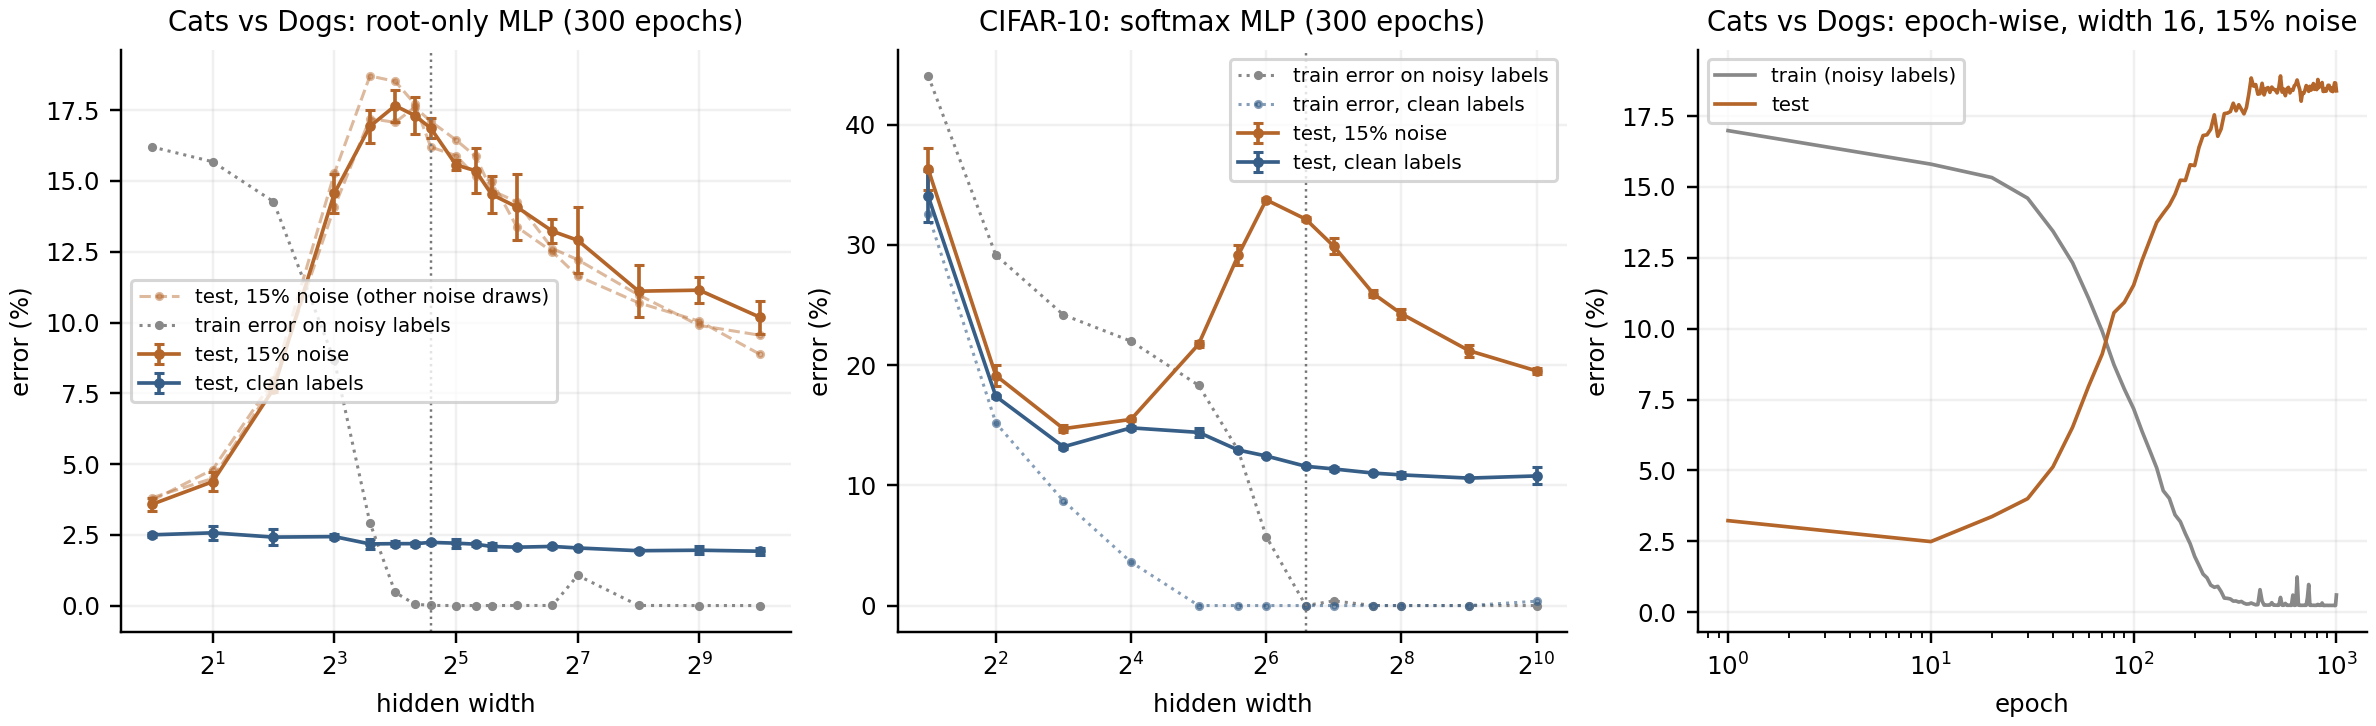
\includegraphics[width=\linewidth]{figures/noise_root_curves.png}
\caption{Fixed-topology root-only networks. Error bars are sample SD over three optimization seeds. Dotted vertical lines mark the first width whose mean noisy-train error is below 0.05\%. Dashed curves (left) are two further noise draws. Right: epoch-wise mean over three seeds.}\label{fig:noiseroot}
\end{figure}
\begin{table}[H]\centering\small
\caption{Root-only width sweeps (mean over three seeds; test SD in parentheses). Bold marks the best width before the peak and the peak.}
\begin{tabular}{lrrrrrr}\toprule
& & & \multicolumn{2}{c}{15\% label noise} & \multicolumn{2}{c}{Clean labels}\\\cmidrule(lr){4-5}\cmidrule(lr){6-7}
Data & Width & Params & Train err.\ (\%) & Test err.\ (\%) & Train err.\ (\%) & Test err.\ (\%)\\\midrule
C/D & 1 & 579 & 16.21 & \textbf{3.58} (0.22) & 0.45 & 2.50 \\
C/D & 4 & 2,313 & 14.27 & 7.65 (0.09) & 0.10 & 2.42 \\
C/D & 8 & 4,625 & 8.67 & 14.56 (0.68) & 0.04 & 2.44 \\
C/D & 12 & 6,937 & 2.93 & 16.93 (0.58) & 0.02 & 2.18 \\
C/D & 16 & 9,249 & 0.47 & \textbf{17.66} (0.57) & 0.01 & 2.19 \\
C/D & 20 & 11,561 & 0.05 & 17.31 (0.65) & 0.00 & 2.19 \\
C/D & 24 & 13,873 & 0.01 & 16.87 (0.36) & 0.00 & 2.23 \\
C/D & 32 & 18,497 & 0.00 & 15.57 (0.16) & 0.00 & 2.21 \\
C/D & 64 & 36,993 & 0.01 & 14.08 (1.16) & 0.00 & 2.06 \\
C/D & 128 & 73,985 & 1.07 & 12.91 (1.17) & 0.00 & 2.04 \\
C/D & 256 & 147,969 & 0.01 & 11.11 (0.92) & 0.00 & 1.94 \\
C/D & 1024 & 591,873 & 0.00 & 10.18 (0.58) & 0.00 & 1.92 \\
\midrule
C10 & 2 & 1,184 & 44.05 & 36.29 (1.74) & 32.55 & 34.03 \\
C10 & 4 & 2,358 & 29.15 & 19.13 (0.89) & 15.19 & 17.40 \\
C10 & 8 & 4,706 & 24.18 & \textbf{14.71} (0.28) & 8.70 & 13.20 \\
C10 & 16 & 9,402 & 21.99 & 15.48 (0.14) & 3.61 & 14.78 \\
C10 & 32 & 18,794 & 18.31 & 21.73 (0.26) & 0.00 & 14.40 \\
C10 & 48 & 28,186 & 12.92 & 29.12 (0.83) & 0.00 & 12.93 \\
C10 & 64 & 37,578 & 5.74 & \textbf{33.75} (0.16) & 0.00 & 12.44 \\
C10 & 96 & 56,362 & 0.00 & 32.14 (0.18) & 0.00 & 11.58 \\
C10 & 128 & 75,146 & 0.39 & 29.88 (0.68) & 0.00 & 11.36 \\
C10 & 256 & 150,282 & 0.00 & 24.27 (0.44) & 0.00 & 10.87 \\
C10 & 512 & 300,554 & 0.00 & 21.20 (0.51) & 0.00 & 10.60 \\
C10 & 1024 & 601,098 & 0.00 & 19.51 (0.27) & 0.36 & 10.78 \\
\bottomrule

\end{tabular}\label{tab:noiseroot}
\end{table}
\textbf{The CIFAR-10 softmax MLP shows the complete decrease--increase--decrease curve} (Figure~\ref{fig:noiseroot}, middle). This result belongs to the single softmax MLP, not to the correction-tree architecture, which is treated in Section~\ref{sec:noisetree}. Test error first falls from 36.3\% to 14.7\% at width 8, then rises to 33.8\% at width 64, where the network fits all but 5.7\% of the noisy labels, and falls again once it interpolates, to 19.5\% at width 1024. The peak sits just before the first width at which every seed fits the noisy labels exactly (width 96, about $5.6\times10^4$ parameters for 45,000 examples), as the double-descent account predicts. The clean control has a small bump at its own interpolation point (13.2\% at width 8, 14.8\% at width 16, then 10.6\% at width 512); noise turns this 1.6-point bump into a 19-point peak.

\textbf{Cats vs Dogs shows the peak and the second descent but not the first descent.} Width 1 is already the best model (3.6\%), because the pretrained features make the task almost linearly separable. Test error then rises to 17.7\% at width 16, where noisy-label fit is nearly complete, and falls to 10.2\% at width 1024. Two other noise draws give the same shape (peaks of 18.7\% and 17.6\%; 8.9\% and 9.6\% at width 1024), while the clean control decreases overall from 2.5\% to 1.9\%, with small reversals but no peak. The noise therefore causes the peak. Epoch-wise, width 16 reaches its best test error (2.5\%) after about 10 epochs and degrades to 18.4\% as it memorizes the flipped labels; no second epoch-wise descent occurs within 1000 epochs.

Overparameterization recovers only part of the damage: the widest noisy models remain far worse than the clean ones (10.2\% versus 1.9\%; 19.5\% versus 10.6\%).

\subsection{The correction tree under noise}\label{sec:noisetree}
\begin{figure}[H]\centering
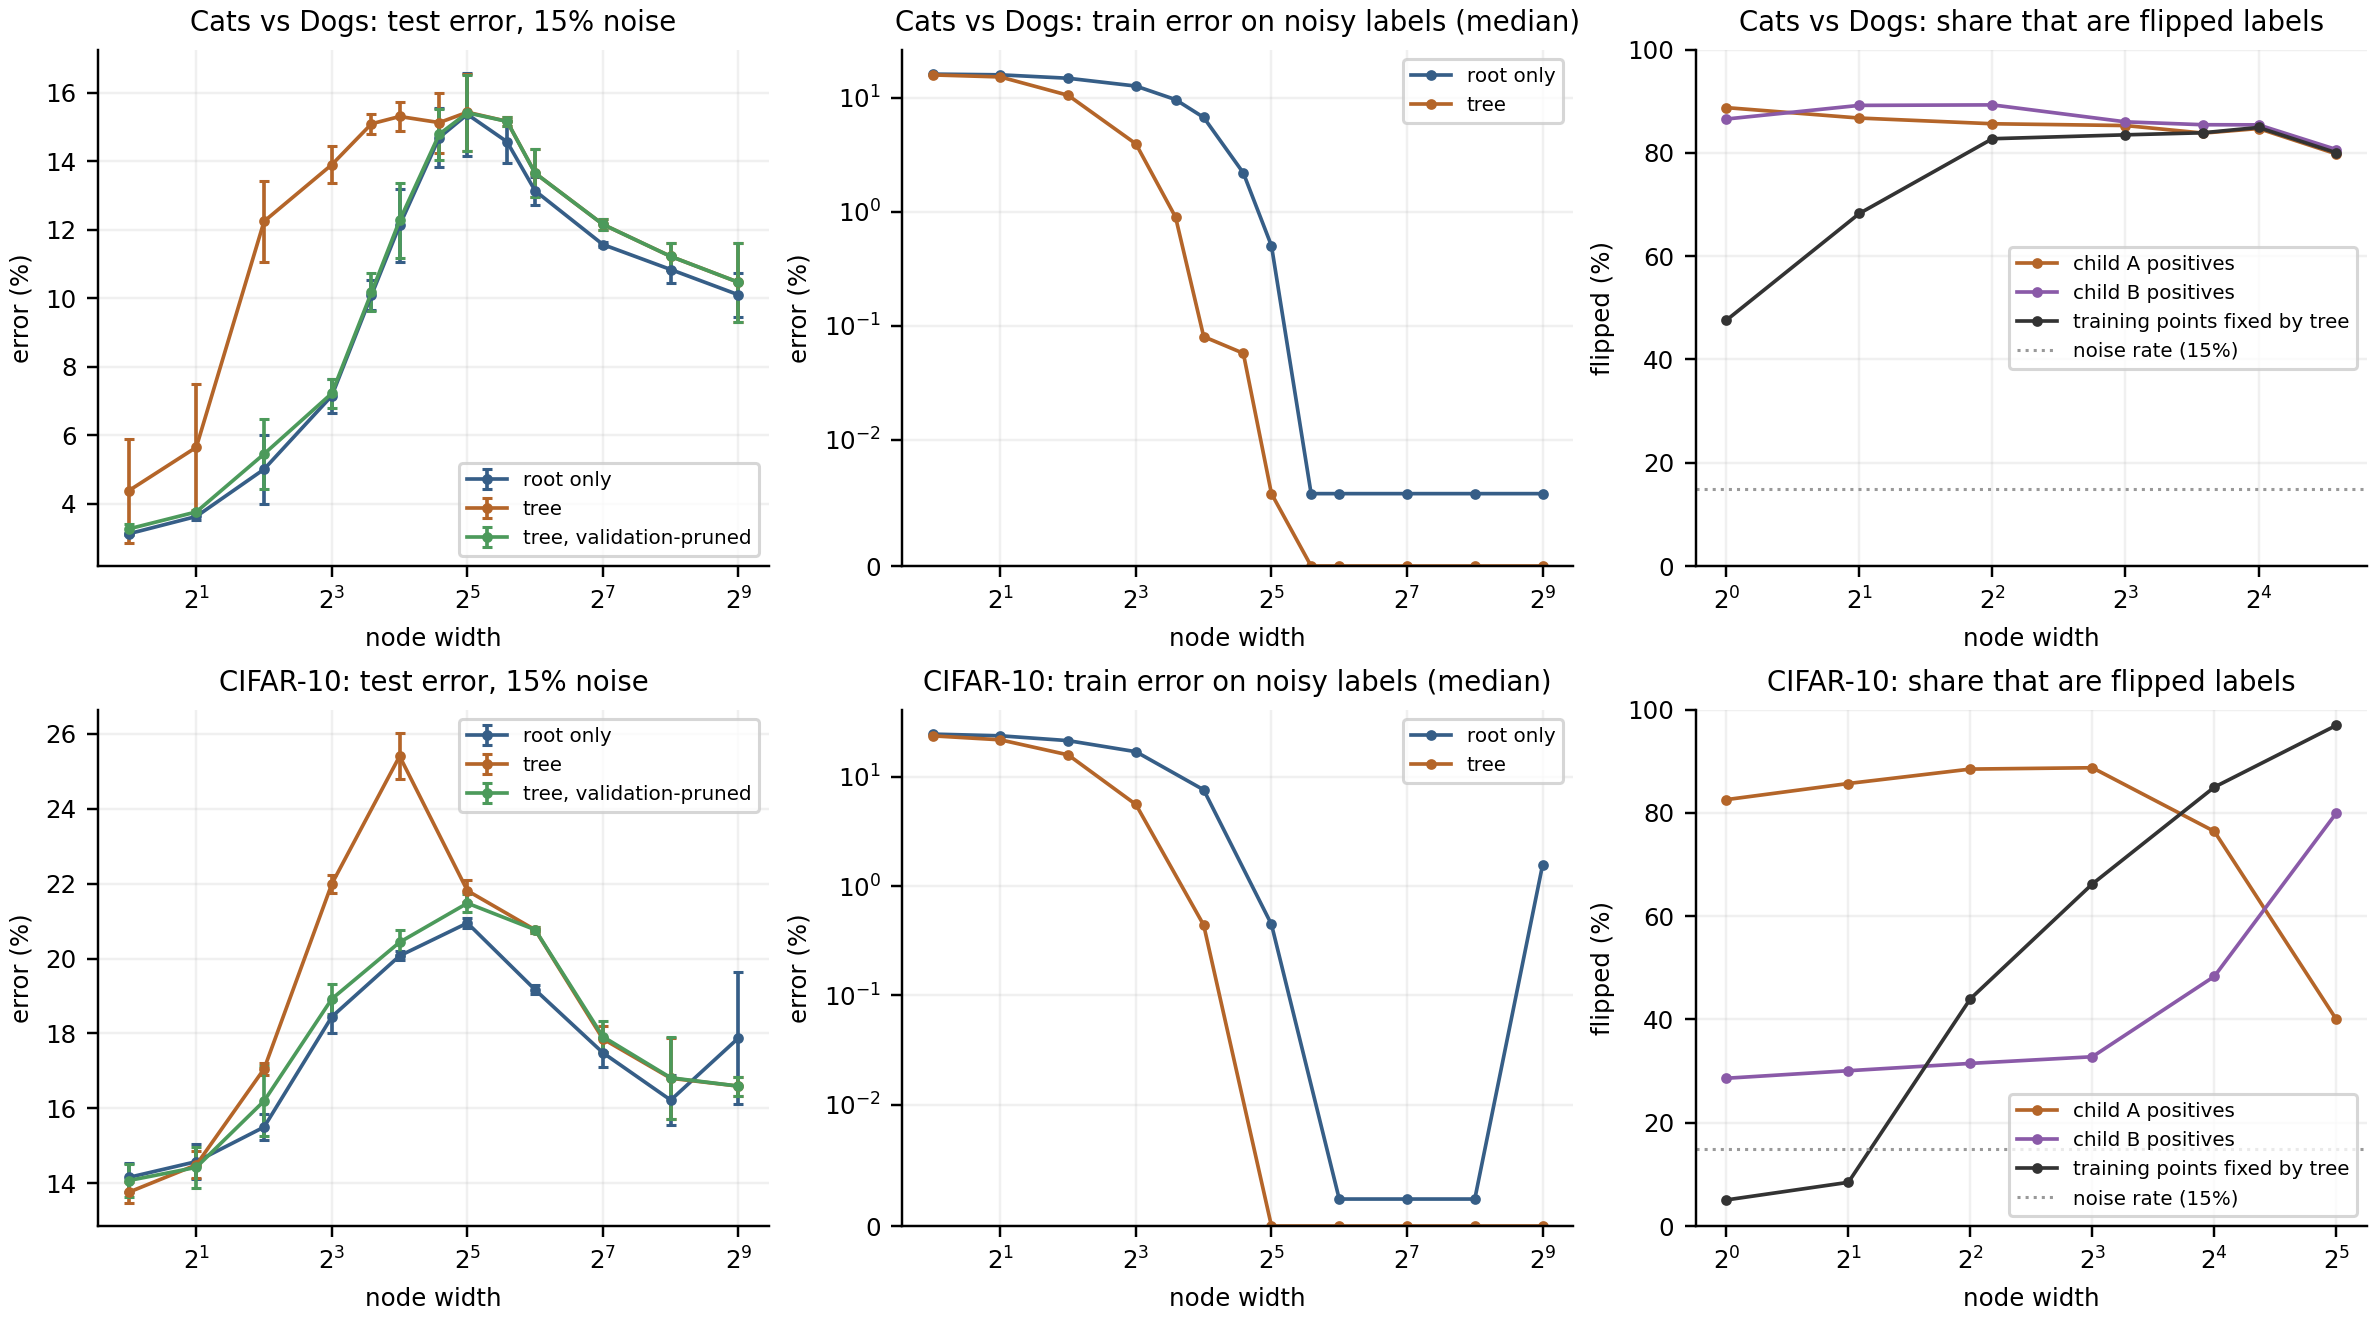
\includegraphics[width=\linewidth]{figures/noise_tree_curves.png}
\caption{Correction trees with 15\% label noise (three seeds). Left: test error of the root-only model, the tree and the validation-pruned tree. Middle: median training error on the noisy labels. Right: share of flipped labels among the positive targets of the roots' children and among the training points the tree fixes, shown only where every root-only run has at least 100 noisy-train errors.}\label{fig:noisetree}
\end{figure}
\begin{table}[H]\centering\small
\caption{Correction trees with 15\% label noise: mean test error (\%) over three seeds, mean noisy-train errors, and the percentage of flipped labels among child-A positive targets / among training points fixed by the tree (``--'' where the root has too few errors to measure).}
\begin{tabular}{lrrrrrrrc}\toprule
Data & Width & Root & Tree & Pruned (orig.) & Pruned (val.) & Root train err. & Tree train err. & Flipped A / fixed\\\midrule
C/D & 1 & 3.12 & 4.38 & 4.41 & 3.27 & 2,833 & 2,775 & 89 / 48 \\
C/D & 4 & 5.01 & 12.25 & 12.07 & 5.46 & 2,599 & 1,861 & 86 / 83 \\
C/D & 8 & 7.16 & 13.90 & 13.90 & 7.23 & 2,238 & 671 & 85 / 83 \\
C/D & 12 & 10.09 & 15.10 & 15.10 & 10.17 & 1,706 & 152 & 84 / 84 \\
C/D & 16 & 12.13 & 15.31 & 15.31 & 12.27 & 1,204 & 17 & 85 / 85 \\
C/D & 24 & 14.70 & 15.13 & 15.13 & 14.79 & 391 & 10 & 80 / 80 \\
C/D & 32 & 15.37 & 15.43 & 15.43 & 15.42 & 74 & 1 & -- \\
C/D & 64 & 13.14 & 13.65 & 13.65 & 13.65 & 1 & 0 & -- \\
C/D & 128 & 11.57 & 12.16 & 12.16 & 12.16 & 1 & 0 & -- \\
C/D & 512 & 10.10 & 10.47 & 10.47 & 10.47 & 1 & 0 & -- \\
\midrule
C10 & 1 & 14.15 & 13.76 & 13.69 & 14.07 & 11,165 & 10,674 & 83 / 5 \\
C10 & 2 & 14.58 & 14.49 & 14.35 & 14.42 & 10,687 & 9,819 & 86 / 8 \\
C10 & 4 & 15.50 & 17.05 & 17.05 & 16.20 & 9,639 & 7,056 & 88 / 44 \\
C10 & 8 & 18.45 & 22.00 & 21.99 & 18.92 & 7,627 & 2,505 & 89 / 66 \\
C10 & 16 & 20.07 & 25.41 & 25.41 & 20.44 & 3,430 & 202 & 76 / 85 \\
C10 & 32 & 20.95 & 21.81 & 21.82 & 21.48 & 195 & 0 & 40 / 97 \\
C10 & 64 & 19.17 & 20.77 & 20.77 & 20.77 & 2 & 0 & -- \\
C10 & 128 & 17.48 & 17.85 & 17.85 & 17.91 & 68 & 0 & -- \\
C10 & 256 & 16.22 & 16.80 & 16.82 & 16.82 & 3 & 0 & -- \\
C10 & 512 & 17.88 & 16.59 & 16.59 & 16.59 & 563 & 0 & -- \\
\bottomrule

\end{tabular}\label{tab:noisetree}
\end{table}
\textbf{The tree also shows a peak followed by descent.} Test error rises from 4.4\% to 15.4\% at width 32 and falls to 10.5\% at width 512 on Cats vs Dogs, and rises from 13.8\% to 25.4\% at width 16 and falls to 16.6\% at width 512 on CIFAR-10. The corrections add capacity: the tree fits the noisy labels at much smaller widths than its own root (CIFAR-10 width 16: about 200 remaining noisy-train errors against 3,430 for the root). On CIFAR-10 the tree's peak therefore moves from width 32 (root-only) to width 16. On Cats vs Dogs both root and tree peak at width 32, but the tree reaches the high-error plateau much earlier (15.1\% at width 12, against 10.1\% for the root). This is consistent with the effective-complexity view of double descent \cite{dd}, in which the peak tracks when the \emph{whole} model can fit the noise.

\textbf{Under noise, the children learn the noise.} Children are trained on their parent's mistakes. When labels are noisy those mistakes are mostly flipped labels: below the interpolation threshold (widths up to 24 on Cats vs Dogs and 16 on CIFAR-10), 76--89\% of child-A positive targets are flipped, against a 15\% noise rate. On Cats vs Dogs, 80--85\% of the training points the tree fixes at widths 4--24 are flipped labels, and the tree is worse than its root at every width (for example 13.9\% against 7.2\% at width 8). CIFAR-10 shows the contrast between helpful and harmful corrections. At widths 1--2 the root underfits the real signal, only 5--8\% of the fixed points are flipped, and the tree is slightly \emph{better} than its root (13.8\% against 14.2\% at width 1). From width 4 onward the fixed points are increasingly flipped labels (44\%, 66\%, 85\%, 97\%) and the tree becomes worse (25.4\% against 20.1\% at width 16). The share of flipped labels among the corrections thus helps explain the observed pattern of when the branches help or hurt; it is a descriptive association across these runs, not a tested predictor.

\textbf{Pruning becomes denoising, but only with a validation criterion.} The original pruning rule forbids any loss of training accuracy, so it keeps the children that memorized noise. Its test error stays close to the tree's, especially around the peak; test counts differ in only 6 of 39 Cats vs Dogs runs and 11 of 30 CIFAR-10 runs, by at most 23 test images, mostly at widths 1--4. The validation-only rule removes them: on Cats vs Dogs all but one of the 39 runs return to the single root node, and test error falls back to the root's level (13.9\% to 7.2\% at width 8; CIFAR-10 width 16: 25.4\% to 20.4\%). Under label noise, minimizing the network and generalizing better therefore coincide, provided the pruning criterion is held-out accuracy rather than training fit. This is consistent with the clean-label finding of Section~\ref{sec:results}: fitting the final training exceptions did not improve test accuracy there either.

\textbf{Two by-products.} First, the child-target groups of Section~\ref{sec:targets} are a promising diagnostic for injected label noise: at width 1 on Cats vs Dogs, 88\% of the root's training errors are flipped labels and they cover 95\% of all flipped labels. This has not been validated as a general noise detector, for example on naturally mislabeled data. Second, the single noisy-train error that wide root-only Cats vs Dogs models keep is one pair of near-identical photographs (\texttt{Dog/9746.jpg} and \texttt{Dog/5733.jpg}, feature distance 0.55 against a median nearest-neighbour distance of 21.2) that the noise gave opposite labels. Exact pixel hashing cannot detect this pair, and the tree fits it with a correction node, which is memorization at its most literal.

\textbf{Caveats.} Six runs ended with unusually many noisy-train errors, consistent with late training instability under Adam without weight decay: Cats vs Dogs root-only width 128 seed 43 (558); CIFAR-10 softmax width 128 seed 29 (520) and clean width 1024 seed 29 (487); and CIFAR-10 tree-sweep root-only width 128 seed 43 (203) and width 512 seeds 29 and 43 (987 and 700). They are kept in all means, which inflates the CIFAR root-only test error at width 512. The CIFAR root-only curve (single softmax MLP, 300 epochs) and the CIFAR tree sweep (ten one-vs-rest roots, 100 epochs per node) differ in architecture and training length, so their peak widths are not directly comparable. One noise rate is studied, the tree and CIFAR-10 sweeps use one noise draw, and the three seeds measure optimization variability only.
